\section{Hypothesentests}

\subsection{Rationale Erklärungen}

\subsubsection{Was ist wahr?}

Wahr ist, was mit der objektiven Realität übereinstimmt


\subsubsection{Rationale Erklärung}

\begin{enumerate}
	\item Erklärungen müssen falsifizierbar sein
	\item Erklärungen müssen mit allen Beobachtungen übereinstimmen
\end{enumerate}


\subsection{Grundätzliche Testmethode}

\begin{minipage}{0.35\columnwidth}
	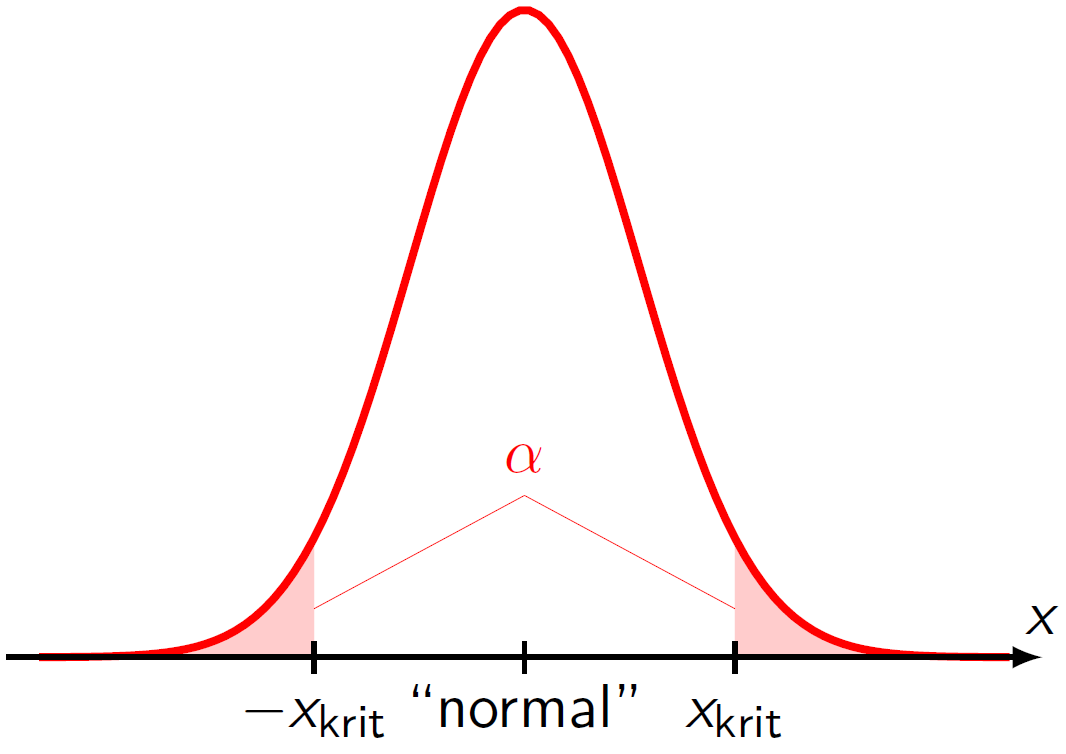
\includegraphics[width=\columnwidth]{images/vorgehen_hypothesentest.png}
\end{minipage}
\hfill
\begin{minipage}{0.6\columnwidth}
	\begin{enumerate}
		\item Nullhypothese $H_0$ formulieren 
		\item Messgrösse bestimmen, mit der $H_0$ getestet werden kann (Teststatistik)
		\item Verteilung der Messgrösse ermitteln
		\item Parameter der Verteilung schätzen
		\item Kritischen Wert für die Testgrösse bestimmen, der nur mit Wahrscheinlichkeit  $\alpha$ überschritten wird.
		\item Ist die Messgrösse im vorliegenden Experiment 'unwahrscheinlich gross? \\
			\textrightarrow\ $H_0$ verwerfen
	\end{enumerate}
\end{minipage}


\subsection{Vorgehen Hypothesentest}

\begin{tabular}{ll}
	$H_0$	& Nullhypothese 'nichts besonderes' (zu widerlegen!)							\\
	$H_1$ 	& Alternativhypothese \textrightarrow\ \textbf{Genau das Gegenteil} von $H_0$
\end{tabular}


\subsubsection{Vorgehen (!)}

\begin{enumerate}
	\item Nullhypothese $H_0$ und Alternativhypothese $H_1$ 
	\item Testgrösse und Verteilung (Testmethode) unter der Annahme der Nullhypothese $H_0$ \\
		\textrightarrow\ Testmethode wählen gemäss Abschnitt \ref{Wahl der richtigen Testmethode}
	\item Wahl des Signifikanzniveaus $\alpha$
	\item Kritischer Wert für Testgrösse, die nur mit Wahrscheinlichkeit $\alpha$ erreicht wird 
	\item Testgrösse $>$ kritischer Wert \textrightarrow\ Nullhypothese $H_0$ \textbf{verwerfen}
\end{enumerate}


\subsubsection{Einschränkungen}

\begin{itemize}
	\item Alternative muss die Negation der Nullhypothese sein \\
		(Fehschluss des falschen Dilemmas)
	\item Es kann viele Möglichkeiten der Widerlegung der Nullhypothese geben
	\item Wenn ein Test scheitert, heisst das nicht, dass die Nullhypothese wahr ist, sondern nur, dass sie noch nicht widerlegt werden konnte 
\end{itemize}


\subsection{Fehlerarten}

\myul{\textbf{Fehler 1. Art}}

\vspace{0.1cm}

Nullhypothese verworfen, obwohl wahr (zufallsbedingt unwahrscheinlicher Wert der Teststatistik, falsch positives Ergebnis) \\
\textbf{\textrightarrow\ Fehler 1. Art tritt mit Wahrscheinlichkeit $\bm{\alpha}$ auf}

\vspace{0.2cm}

\myul{\textbf{Fehler 2. Art}}

\vspace{0.1cm}

Nullhypothese nicht verworfen, obwohl falsch (falsch negatives Ergebnis)

\vspace{0.2cm}


\subsubsection{Typische Werte für $\bm{\alpha}$ }

\begin{center}
	\begin{tabular}{l | l}
		$\alpha$ 		& 							\\
		\hline
		$\bm{0.05}$		& \textbf{'signifikant'} 	\\
		\hline
		$0.01$ 			& 'hoch signifikant' 		\\
		$0.001$ 		& 'hoch signifikant' 		\\
		\hline
	\end{tabular}
\end{center}


\example{Hypothesentest: Faire Münze}

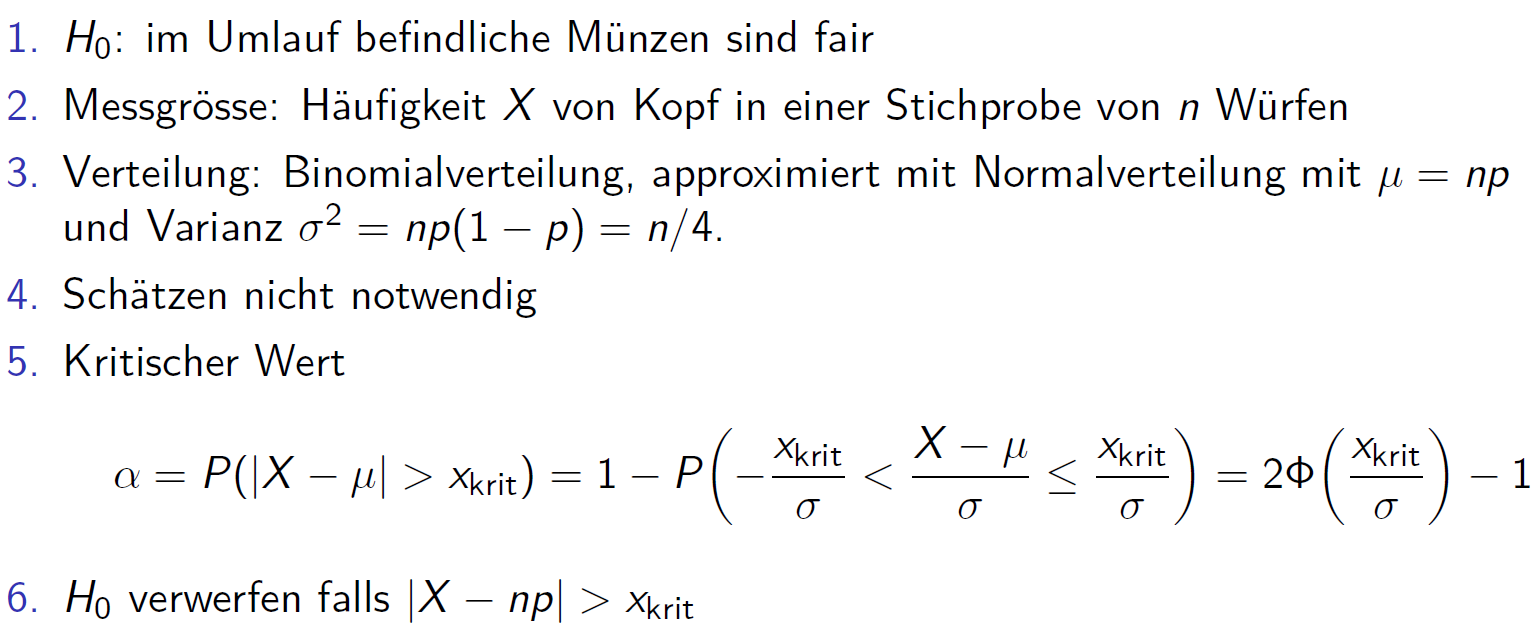
\includegraphics[width=\columnwidth]{images/beispiel_faire_muenze.png}


\subsection{Wahl der richtigen Testmethode}
\label{Wahl der richtigen Testmethode}

\begin{itemize}
	\setlength\itemsep{5pt}
	\item Wahrscheinlichkeiten (diskrete Verteilung mit endlicher Anzahl Versuchsausgänge) prüfen \\
 		\textrightarrow\ $\chi^2$-Test 
 
 	\item Prüfen auf (gleichen) Erwartungswert $E(X)$ \\
	 \textrightarrow\ $t$-Test 
 
 	\item Abweichung von Mittelwert prüfen \\
 		\textrightarrow\ Normalverteilung 
 
 	\item Prüfung auf Abweichung von Verteilungsfunktion $F(x)$ \\
		\textrightarrow\ Kolmogorov-Smirnov-Test 
\end{itemize}


\subsection[Hypothesentest mit t-Verteilung]{Hypothesentest mit $t$-Verteilung}

\subsubsection{Nullhypothese $\bm{H_0}$}

Die Stichproben $X_1,\, \ldots , \, X_n \text{ und } Y_1, \, \ldots , \, Y_m$ mit gleicher Varianz haben den gleichen Erwartungswert. 


\subsubsection{Teststatistik}

$$ t = \frac{\overline{X} - \overline{Y}}{\sqrt{(n-1) S_X^2 + (m-1) S_Y^2}} \, \sqrt{\frac{n \, m \, (n+m-2)}{n+m}} $$

ist $t$-verteilt mit $k = m+n-2$ Freiheitsgraden


\subsubsection{Parameter schätzen}

\begin{minipage}[c]{0.48\columnwidth}
	$$ \overline{X} = \frac{X_1 + \ldots + X_n}{n} $$
\end{minipage}
\hfill
\begin{minipage}[c]{0.48\columnwidth}
	$$ S_X^2 = \frac{1}{n-1} \sum\limits_{i=1}^n (X_i - \overline{X})^2 $$
\end{minipage}

\vspace{0.2cm}

\begin{minipage}[c]{0.48\columnwidth}
	$$ \overline{Y} = \frac{Y_1+ \ldots + Y_m}{m} $$
\end{minipage}
\hfill
\begin{minipage}[c]{0.48\columnwidth}
	$$ S_Y^2 = \frac{1}{m-1} \sum\limits_{i=1}^m (Y_i - \overline{Y})^2 $$
\end{minipage}

\vspace{0.2cm}

\textrightarrow\ Tabelle $t$-Verteilung siehe Abschnitt \ref{Quantilen der t-Verteilung}


\subsection[p-Value]{$p$-Value}

\begin{minipage}[c]{0.35\columnwidth}
	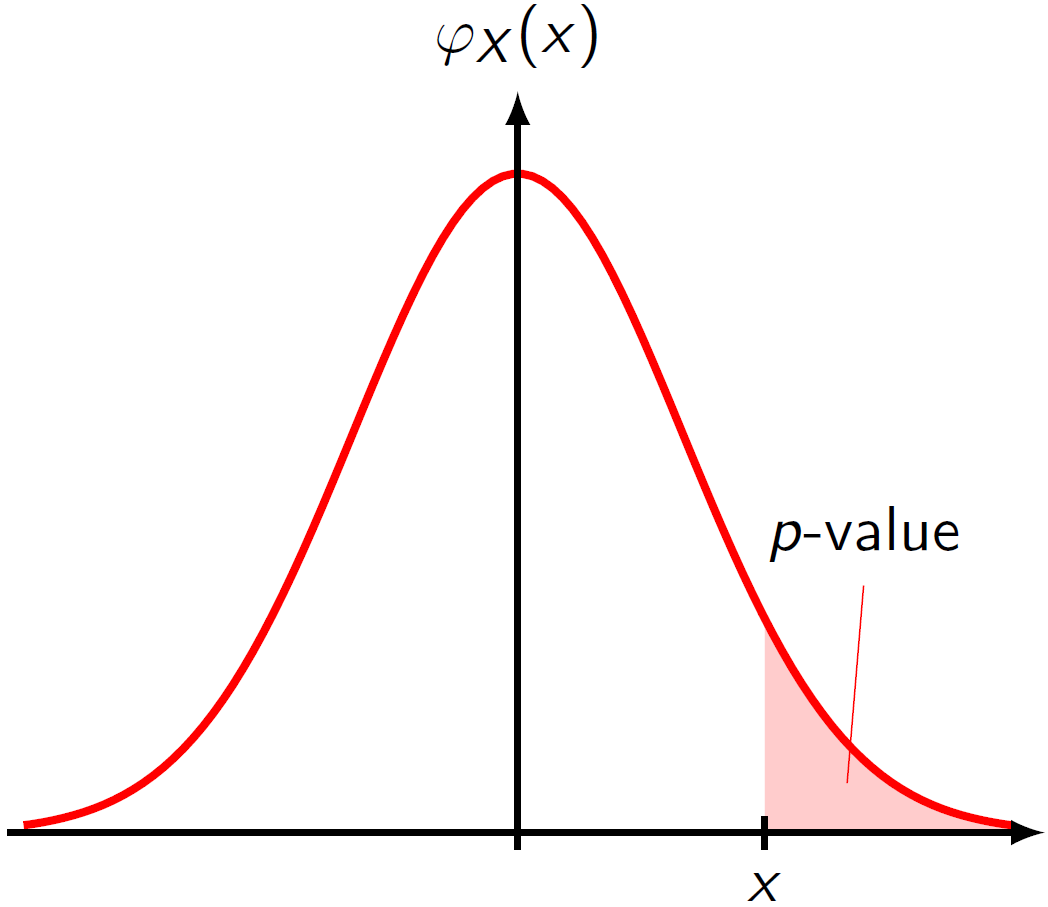
\includegraphics[width=\columnwidth]{images/p-value.png}
\end{minipage}
\hfill
\begin{minipage}[c]{0.58\columnwidth}
	Der $p$-Value beschreibt die \textbf{Wahrscheinlichkeit, einen Wert $> x$} zu erhalten
	$$ \boxed{ p-\text{Value} = \alpha = P(X > x) = 1 - F(x) } $$

	\myul{\textbf{Interpretation}}

	\vspace{0.1cm}

	$p$-Values beschreiben Wahrscheinlichkeit für Fehler 1. Art
\end{minipage}


\subsection{$\chi^2$-Test}

Testen einer \textbf{diskreten} Verteilung \\
\textbf{Mehrere Versuchsausgänge} (endliche Anzahl) möglich! 

\vspace{0.2cm}

Diskrete Verteilung $P(X = x_i) = p_i$ mit $n_i$ Beobachtungen für jeden Wert

\vspace{0.2cm}

\begin{enumerate}
	\item $H_0$: Beobachtete Häufigkeiten $n_i$ entsprechen Wahrscheinlichkeiten $p_i$ 
	\item Messgrösse: Diskrepanz $D$
	\item Verteilung: $\chi^2$-Verteilung mit $k = d-1$ Freiheitsgraden \\
		$d = $ Anzahl mögliche Versuchsausgänge
	\item Signifikanzniveau $\alpha$ wählen
	\item Schätzen: nicht nötig
	\item Kritischer Wert: $D_{\rm krit}$ aus der $\chi^2$-Tabelle (Abschnitt \ref{Quantilen der chi2-Verteilung})
	\item $H_0$ verwerfen wenn $D > D_{\rm krit}$
\end{enumerate}

\vspace{0.2cm}

\textbf{Einschränkung:} $n_i \geq 5$ (zentraler Grenzwertsatz)


\subsubsection{Messgrösse: Diskrepanz $D$}

$$ \boxed{ D = \sum\limits_{i = 1}^d \frac{(n_i - n \, p_i)^2}{n \, p_i}} $$

\begin{tabular}{ll}
	$n$ 	& Totale Anzahl Versuche 								\\
	$n_i$ 	& Wie oft Ergebnis $i$ eingetreten ist 					\\
	$p_i$ 	& Wahrscheinlichkeit $P(X = x_i)$ gemäss Nullhypothese 
\end{tabular}


\subsection{Kolmogorov-Smirnov-Test}

\textbf{Frage: } 'Folgt eine Zufallsvariable einer gegebenen Verteilung?' \\
\textbf{\textrightarrow\ Daten $\bm{x_i}$ müssen zuerst \myul{aufsteigend} sortiert werden!}

\vspace{0.2cm}

\begin{minipage}{0.4\columnwidth}
	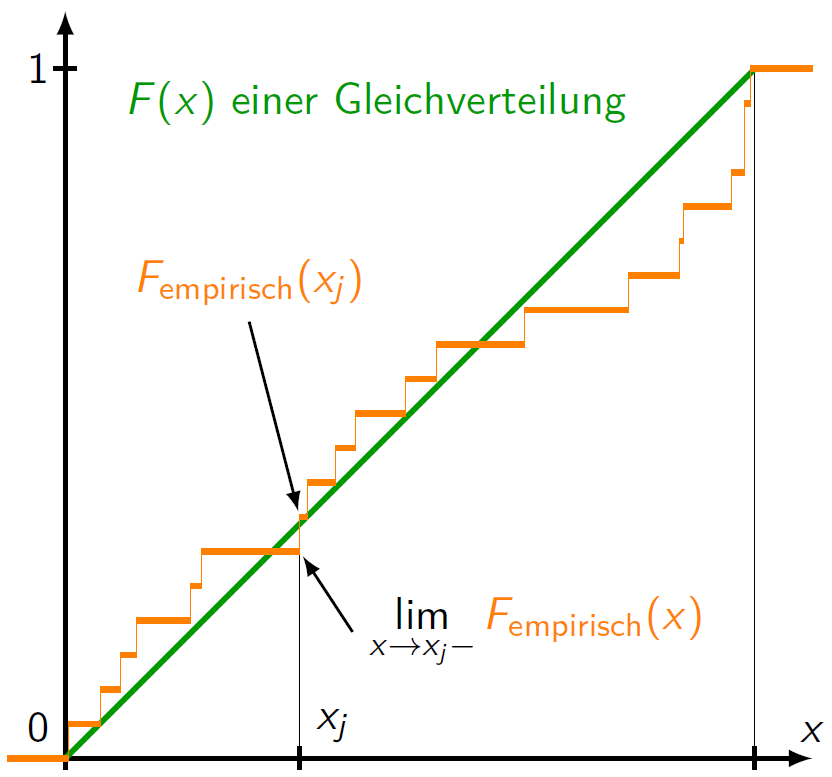
\includegraphics[width=\columnwidth]{images/empirische_verteilungsfunktion.png}
\end{minipage}
\hfill
\begin{minipage}{0.58\columnwidth}
	Daten: $x_1 \leq \ldots \leq x_j \leq \ldots \leq x_n$ 

	$$ \boxed{ \cor{F_{\text{empirisch}}(x_j)} = \frac{j}{n} } $$
	$$ \boxed{ \lim\limits_{x \to \_j^-} \cor{F_{\text{empirisch}}(x_j)} = \frac{j-1}{n} } $$
\end{minipage}

\vspace{0.2cm}

Abweichung der \cor{empirischen Verteilungsfunktion} von der \cgn{Verteilungsfunktion}: 

$$ \boxed{ K_n^+ = \sqrt{n} \, \mathrm{max}_x(F_{\text{empirisch}}(x) - F(x)) = \sqrt{n} \, \mathrm{max}_j \Big( \frac{j}{n} - F(x_j) \Big)  } $$
$$ \boxed{ K_n^- = \sqrt{n} \, \mathrm{max}_x( F(x) - F_{\text{empirisch}}(x)) = \sqrt{n} \, \mathrm{max}_j \Big( F(x_j) - \frac{j-1}{n} \Big)  } $$

\vspace{0.2cm}

\textrightarrow\ Falls $K_n^+ > K_{\rm krit}$ \textrightarrow\ $H_0$ verwerfen \\
\textrightarrow\ KS-Tabelle siehe Abschnitt \ref{Quantilen für Kolmogorov-Smirnov-Test}


\subsection{Q-Q-Plot}

\textbf{Frage:} 'Gehören zwei Datensätze zur gleichen Verteilung?'

\vspace{0.2cm}

\begin{minipage}{0.3\columnwidth}
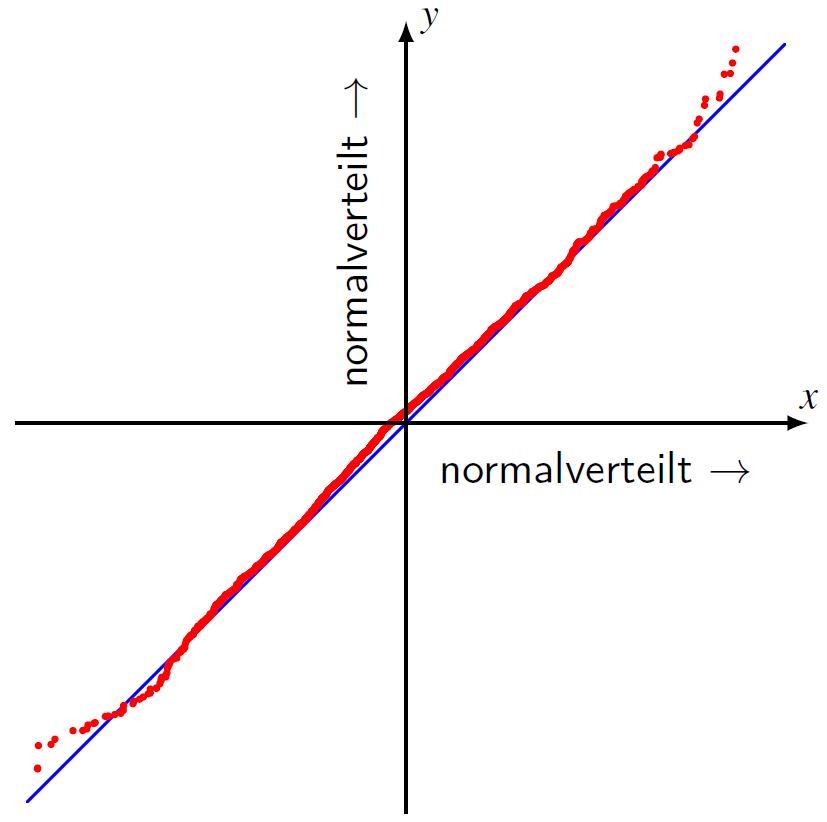
\includegraphics[width=\columnwidth]{images/Q-Q-plot.png}
\end{minipage}
\hfill
\begin{minipage}{0.6\columnwidth}
	\myul{\textbf{Verteilungsvergleich}}

	\vspace{0.2cm}

	\begin{enumerate}
		\setlength\itemsep{5pt}
		\item  \textbf{sortieren} \\
			$x_1 \leq ... \leq ... \leq x_n$ \\
			$y_1 \leq ... \leq ... \leq y_n$ 
		\item Punkte $p_i = (x_i, y_i)$ darstellen 
		\item Gleiche Verteilung, wenn Punkte $P_i$ ungefähr auf einer \textbf{Geraden} liegen 
	\end{enumerate}
\end{minipage}

